\section{Weightless Networks as an Exact Unlearning Substrate}
\label{sec:unlearning}

Section~\ref{sec:unl-mech} explains why deletion is exact for a weightless network and how that exactness can be certified; Section~\ref{sec:unl-setup} states the metrics and baselines; Section~\ref{sec:unl-results} reports four deletion scenarios. Figure~\ref{fig:trade} previews the result as a deletion trade surface on which the weightless network and the exact baselines occupy different corners.

\begin{figure}[t]
  \centering
  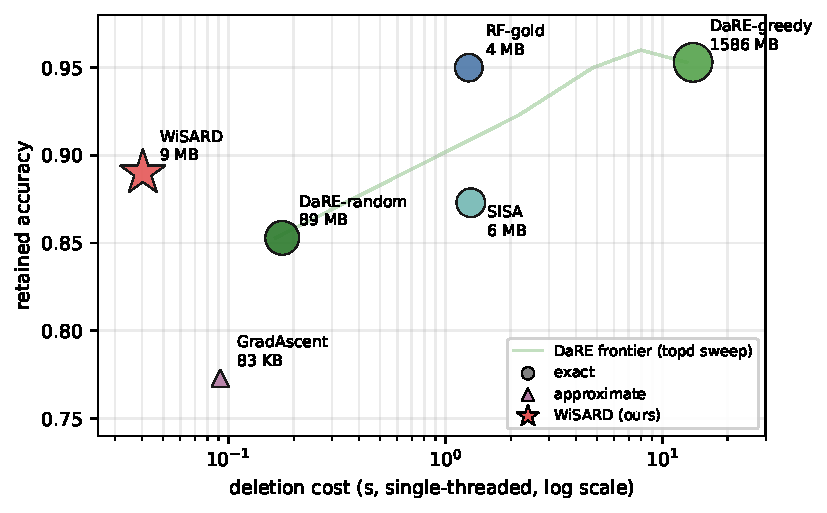
\includegraphics[width=0.82\textwidth]{figures/trade_surface.pdf}
  \caption{Deletion cost versus retained accuracy for a right-to-be-forgotten class erasure, timed single-threaded. Marker area encodes the memory a method holds to support deletion; circles are exact methods and the triangle is the approximate baseline. The weightless network occupies the latency-first corner (40~ms, 0.89, 9.3~MB) and the greedy DaRE forest the accuracy-first corner (13.9~s, 0.95, 1.6~GB); sweeping the DaRE frontier, no setting reaches both the weightless network's cost and its accuracy.}
  \label{fig:trade}
\end{figure}

\subsection{Exact deletion by construction}
\label{sec:unl-mech}

A weightless network trains by addition. Each training example increments a fixed set of RAM counters, one per address it activates, independently of every other example, so the trained model is the sum of its per-example contributions. Deleting an example is therefore subtraction: decrementing exactly the counters it incremented returns the model to the state it would have reached without that example, bit for bit. The operation is \texttt{untrain}, already provided by the wisardpkg library; it is exact by construction, with no substructure to rebuild as in a forest and no weight to nudge as in gradient descent.

This exactness can be certified directly. Because deletion restores the counters to their never-incremented values, the vote memory after unlearning a batch is identical to that of a model that never saw the batch, and the two can be compared cell by cell; in our experiments the maximum counter difference is zero. No weighted model offers this check: the influence of one example cannot be read off a forest's splits or a network's weights, so its removal can only be trusted by construction, retrained-and-compared at full cost, or probed statistically. We adopt the statistical probe, the membership-inference attack, as the common currency that also scores the approximate baseline.

\subsection{Metrics and baselines}
\label{sec:unl-setup}

We ask three questions of each deletion: whether the model behaves as if the data were never seen, what the deletion costs, and whether retained accuracy is preserved. Forgetting is read two ways: the forget effect, the model's accuracy on the deleted data, which a correct deletion drives to chance; and the membership-inference AUC of a confidence-threshold attack, which separates the deleted examples from fresh never-seen examples of the same kind using the unlearned model's confidence, where 0.5 means indistinguishable and above 0.5 a residual leak. Deletion cost is the wall-clock of the deletion alone, measured single-threaded so it reflects algorithmic work rather than core count, together with the memory a method holds to support deletion; retained utility is test accuracy on the data kept.

We compare the weightless network against four baselines on a shared six-class corpus: retraining from scratch on the surviving data, the exact gold standard; SISA, which shards the data and retrains only affected shards; data-removal-enabled (DaRE) forests in their greedy and random regimes, the purpose-built exact-forest method, matched to the gold-standard forest and applied one-vs-rest; and gradient ascent, an approximate method that raises the deleted example's loss in place. The first three are exact; gradient ascent is not.

\subsection{Four deletion scenarios}
\label{sec:unl-results}

Erasing a class is the first request: all Odlaw training rows are deleted, and the model must keep the other five classes intact. Every exact method removes Odlaw completely and drives its membership AUC to 0.5, so the separation is cost (Table~\ref{tab:s1}). The weightless network empties Odlaw's discriminator in 40~ms at its 9.3~MB footprint; retraining rebuilds all 300 trees in 1.28~s, SISA retrains every shard in 1.31~s (class deletion is its worst case, the class being spread across all shards), and the DaRE forest needs 13.9~s and 1.6~GB of cached split statistics to keep the deletion both exact and as accurate as the gold standard. Retained accuracy is 0.89 for the weightless network against the gold standard's 0.95, while gradient ascent is cheap at 92~ms but approximate, paying in utility here as it falls to 0.77. The certificate holds throughout: the scrubbed vote memory is identical to a never-trained one, and Figure~\ref{fig:inside} shows the deletion from inside both models.

\begin{table}[t]
  \centering
  \caption{Class erasure (delete all Odlaw rows), single-threaded. Cost is the deletion wall-clock; accuracy is on the five kept classes; memory is what each method holds to support deletion; a membership AUC of 0.5 is clean forgetting. Best per column in bold.}
  \label{tab:s1}
  \begin{tabular}{lrrrcr}
    \toprule
    Method & Cost (s) & Acc. & Mem.\ (MB) & Exact & MIA \\
    \midrule
    WiSARD (ours)   & \textbf{0.040} & 0.89 & 9.3 & yes & 0.50 \\
    Retrain (gold)  & 1.28 & \textbf{0.95} & \textbf{3.8} & yes & 0.50 \\
    SISA            & 1.31 & 0.87 & 6.3 & yes & 0.50 \\
    DaRE-greedy     & 13.87 & \textbf{0.95} & 1585.7 & yes & 0.50 \\
    DaRE-random     & 0.18 & 0.85 & 89.1 & yes & 0.50 \\
    Gradient ascent & 0.09 & 0.77 & 0.08 & no & 0.48 \\
    \bottomrule
  \end{tabular}
\end{table}

\begin{figure}[t]
  \centering
  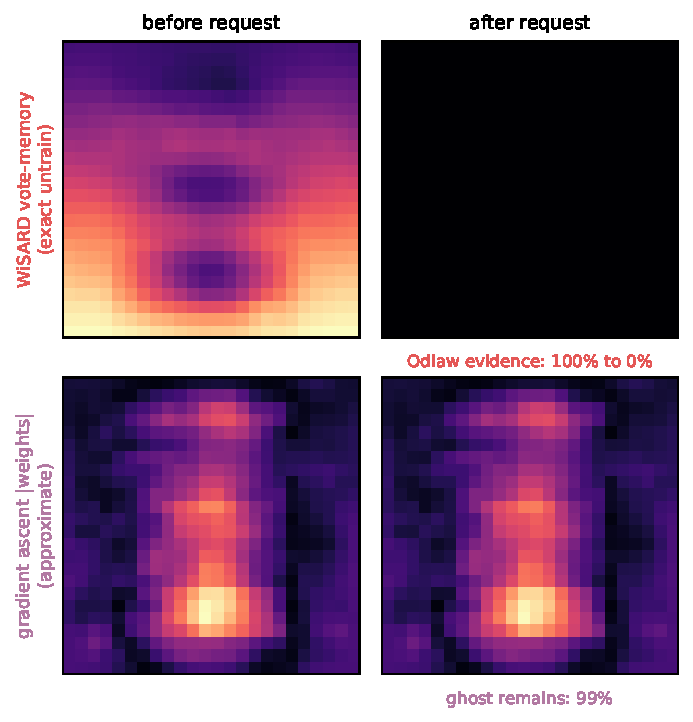
\includegraphics[width=0.60\textwidth]{figures/forgetting_inside.pdf}
  \caption{Forgetting Odlaw, seen from inside each model. Top: the weightless network's back-projected vote memory for Odlaw is a structured imprint before the request and identically zero after \texttt{untrain} (1.16M votes to 0), neighbouring classes unchanged. Bottom: gradient ascent can only push weights down, leaving 99\% of the Odlaw evidence as a structured ghost---the residue that surfaces as a membership-inference leak once the class survives deletion (the poison scenario).}
  \label{fig:inside}
\end{figure}

Removing a poisoned contribution is more discriminating, because the class survives and membership becomes a real question. We inject 100 Wizard patches mislabelled as Waldo, then delete exactly those rows; before deletion the attack separates them well above chance, confirming the model memorised them. The weightless network erases the 100 counters in milliseconds and collapses the membership AUC to 0.5, restoring clean accuracy, while gradient ascent, at comparable cost, leaves the AUC above 0.5---the residual leak the exactness guarantee exists to prevent. The exact methods trace a trade surface, with the weightless network at the latency-first end (tens of milliseconds, 0.89 accuracy, 9.3~MB) and the greedy DaRE forest at the accuracy-first end (matching the gold standard's 0.95, but at roughly 14~s and 1.6~GB); sweeping DaRE's full accuracy-cost frontier, no setting is at once as accurate as the gold standard and as cheap as the weightless deletion.

The cost that matters in deployment is not one deletion but a stream of them. Replaying 30 deletion requests, each removing one contributor's rows, the weightless network's cumulative cost stays flat, because each \texttt{untrain} costs in proportion to the rows deleted and is independent of corpus size and history; the thirtieth request costs what the first did, 0.25~s in total. The exact baselines accumulate: best-case SISA, sharded by contributor so each request hits one shard, still spends 2.5~s, the DaRE forest in its random regime 1.4~s, and gold-standard retraining 27~s, because each request rebuilds a 300-tree model. The constant-versus-linear gap is the deployment argument, and it only widens over a model's lifetime of accumulating requests.

The same primitive defends a detector, not only a classifier. We poison a sliding-window Waldo detector with a distinctive trigger mislabelled as the target, so that before scrubbing every trigger patch is detected as Waldo and the trigger fires the detector in every scene. A single \texttt{untrain} of the poisoned windows removes the backdoor exactly, dropping trigger detection from 1.00 to 0.00 in milliseconds while genuine Waldo detection is untouched. Removing a trojan is the same counter-subtraction as honouring a deletion request, and it extends the exact guarantee from patch classification to spatial detection.
